\let\counterwithout\relax
\let\counterwithin\relax
\documentclass[final]{fhnwreport}       %[mode] = draft or final
\usepackage{color, colortbl}
\definecolor{grau}{gray}{0.9}
\definecolor{hellgrau}{gray}{0.95}
\pagestyle{empty}                             %{class} = fhnwreport, article, 
                                       %          report, book, beamer, standalone
%%---Main Packages-----------------------------------------------------------------------
\usepackage[english, ngerman]{babel}	%Mul­tilin­gual sup­port for LaTeX
\usepackage[T1]{fontenc}				%Stan­dard pack­age for se­lect­ing font en­cod­ings
\usepackage[utf8]{inputenc}				%Ac­cept dif­fer­ent in­put en­cod­ings
\usepackage{lmodern}                    %The newer Font-Set
\usepackage{textcomp}					%LaTeX sup­port for the Text Com­pan­ion fonts
\usepackage{graphicx} 					%En­hanced sup­port for graph­ics
\usepackage{float}						%Im­proved in­ter­face for float­ing ob­jects
\usepackage{ifdraft}                    %Let you check if the doc is in draft mode

%%---Useful Packages---------------------------------------------------------------------
\usepackage[pdftex,dvipsnames]{xcolor}  %Driver-in­de­pen­dent color ex­ten­sions for LaTeX
\usepackage{csquotes}                   %Simpler quoting with \enquote{}
\usepackage{siunitx} 					%A com­pre­hen­sive (SI) units pack­age
\usepackage{listings}					%Type­set source code list­ings us­ing LaTeX
\usepackage[bottom]{footmisc}			%A range of foot­note op­tions
\usepackage{footnote}					%Im­prove on LaTeX's foot­note han­dling
\usepackage{verbatim}					%Reim­ple­men­ta­tion of and ex­ten­sions to LaTeX ver­ba­tim
\usepackage[textsize=footnotesize]{todonotes} %Mark­ing things to do in a LaTeX doc­u­ment

%%---Tikz Packages-----------------------------------------------------------------------
\usepackage{standalone}
\usepackage{tikz}
\usepackage{circuitikz}
\usetikzlibrary{arrows}
\usetikzlibrary{calc}
\usetikzlibrary{intersections}

%%---Math Packages-----------------------------------------------------------------------
\usepackage{amsmath}					%AMS math­e­mat­i­cal fa­cil­i­ties for LaTeX
%\usepackage{amssymb}					%Type­set­ting symbols (AMS style)
%\usepackage{array}						%Ex­tend­ing the ar­ray and tab­u­lar en­vi­ron­ments
%\usepackage{amsthm}					%Type­set­ting the­o­rems (AMS style)

%%---Table Packages----------------------------------------------------------------------
\usepackage{tabularx}					%Tab­u­lars with ad­justable-width columns
%\usepackage{longtable}
\usepackage{multirow}					%Create tab­u­lar cells span­ning mul­ti­ple rows
\usepackage{multicol}					%In­ter­mix sin­gle and mul­ti­ple columns

%%---PDF / Figure Packages---------------------------------------------------------------
\usepackage{pdfpages}					%In­clude PDF doc­u­ments in LaTeX
\usepackage{pdflscape}					%Make land­scape pages dis­play as land­scape
\usepackage{subfig}					    %Fig­ures di­vided into sub­fig­ures

%%---Other Packages----------------------------------------------------------------------
%\usepackage{xargs}                     %De­fine com­mands with many op­tional ar­gu­ments

%%---Bibliography------------------------------------------------------------------------
\usepackage[style=ieee,urldate=comp,backend=biber, natbib=true]{biblatex}
\addbibresource{literature/bibliography.bib}

%%---Main Settings-----------------------------------------------------------------------
\graphicspath{{./graphics/}}			%Defines the graphicspath
%\geometry{twoside=false}				    %twoside=false disables the "bookstyle"
\setlength{\marginparwidth}{2cm}
\overfullrule=5em						%Creates a black rule if text goes over the margins => debugging


%%---User Definitions--------------------------------------------------------------------
%%Tabel-Definitions: (requires \usepackage{tabularx})
\newcolumntype{L}[1]{>{\raggedright\arraybackslash}p{#1}}    %column-width and alignment
\newcolumntype{C}[1]{>{\centering\arraybackslash}p{#1}}
\newcolumntype{R}[1]{>{\raggedleft\arraybackslash}p{#1}}

%%---Optional Package Settings-----------------------------------------------------------
%Listings-Settings: (requires \usepackage{listings}) => Example with Matlab Code
\lstset{language=Matlab,%
    basicstyle=\footnotesize\ttfamily,
    breaklines=false,%
    morekeywords={switch, case, otherwise},
    keywordstyle=\color{Blue},%
    tabsize=2,
    %morekeywords=[2]{1}, keywordstyle=[2]{\color{black}},
    identifierstyle=\color{Black},%
    stringstyle=\color{Purple},
    commentstyle=\color{Green},%
    showstringspaces=false,%without this there will be a symbol in the places where there is a space
    numbers=left,%
    numberstyle={\tiny \color{black}},% size of the numbers
    numbersep=9pt, % this defines how far the numbers are from the text
    %emph=[1]{word1, word2,...},emphstyle=[1]\color{red}
}							
			                %loads all packages, definitions and settings												
\title{Kleinwasserkraftwerk}          	%Project Title
\author{Dossier}          		%Document Type => Technical Report, ...
\date{Windisch, 18.12.2018}             %Place and Date


\begin{document}

%%---TITLEPAGE---------------------------------------------------------------------------
\selectlanguage{ngerman}                %ngerman or english
\maketitle

\vspace*{-1cm}						    %compensates the space after the date line.
\vfill
\begin{figure} [H]
	\centering
	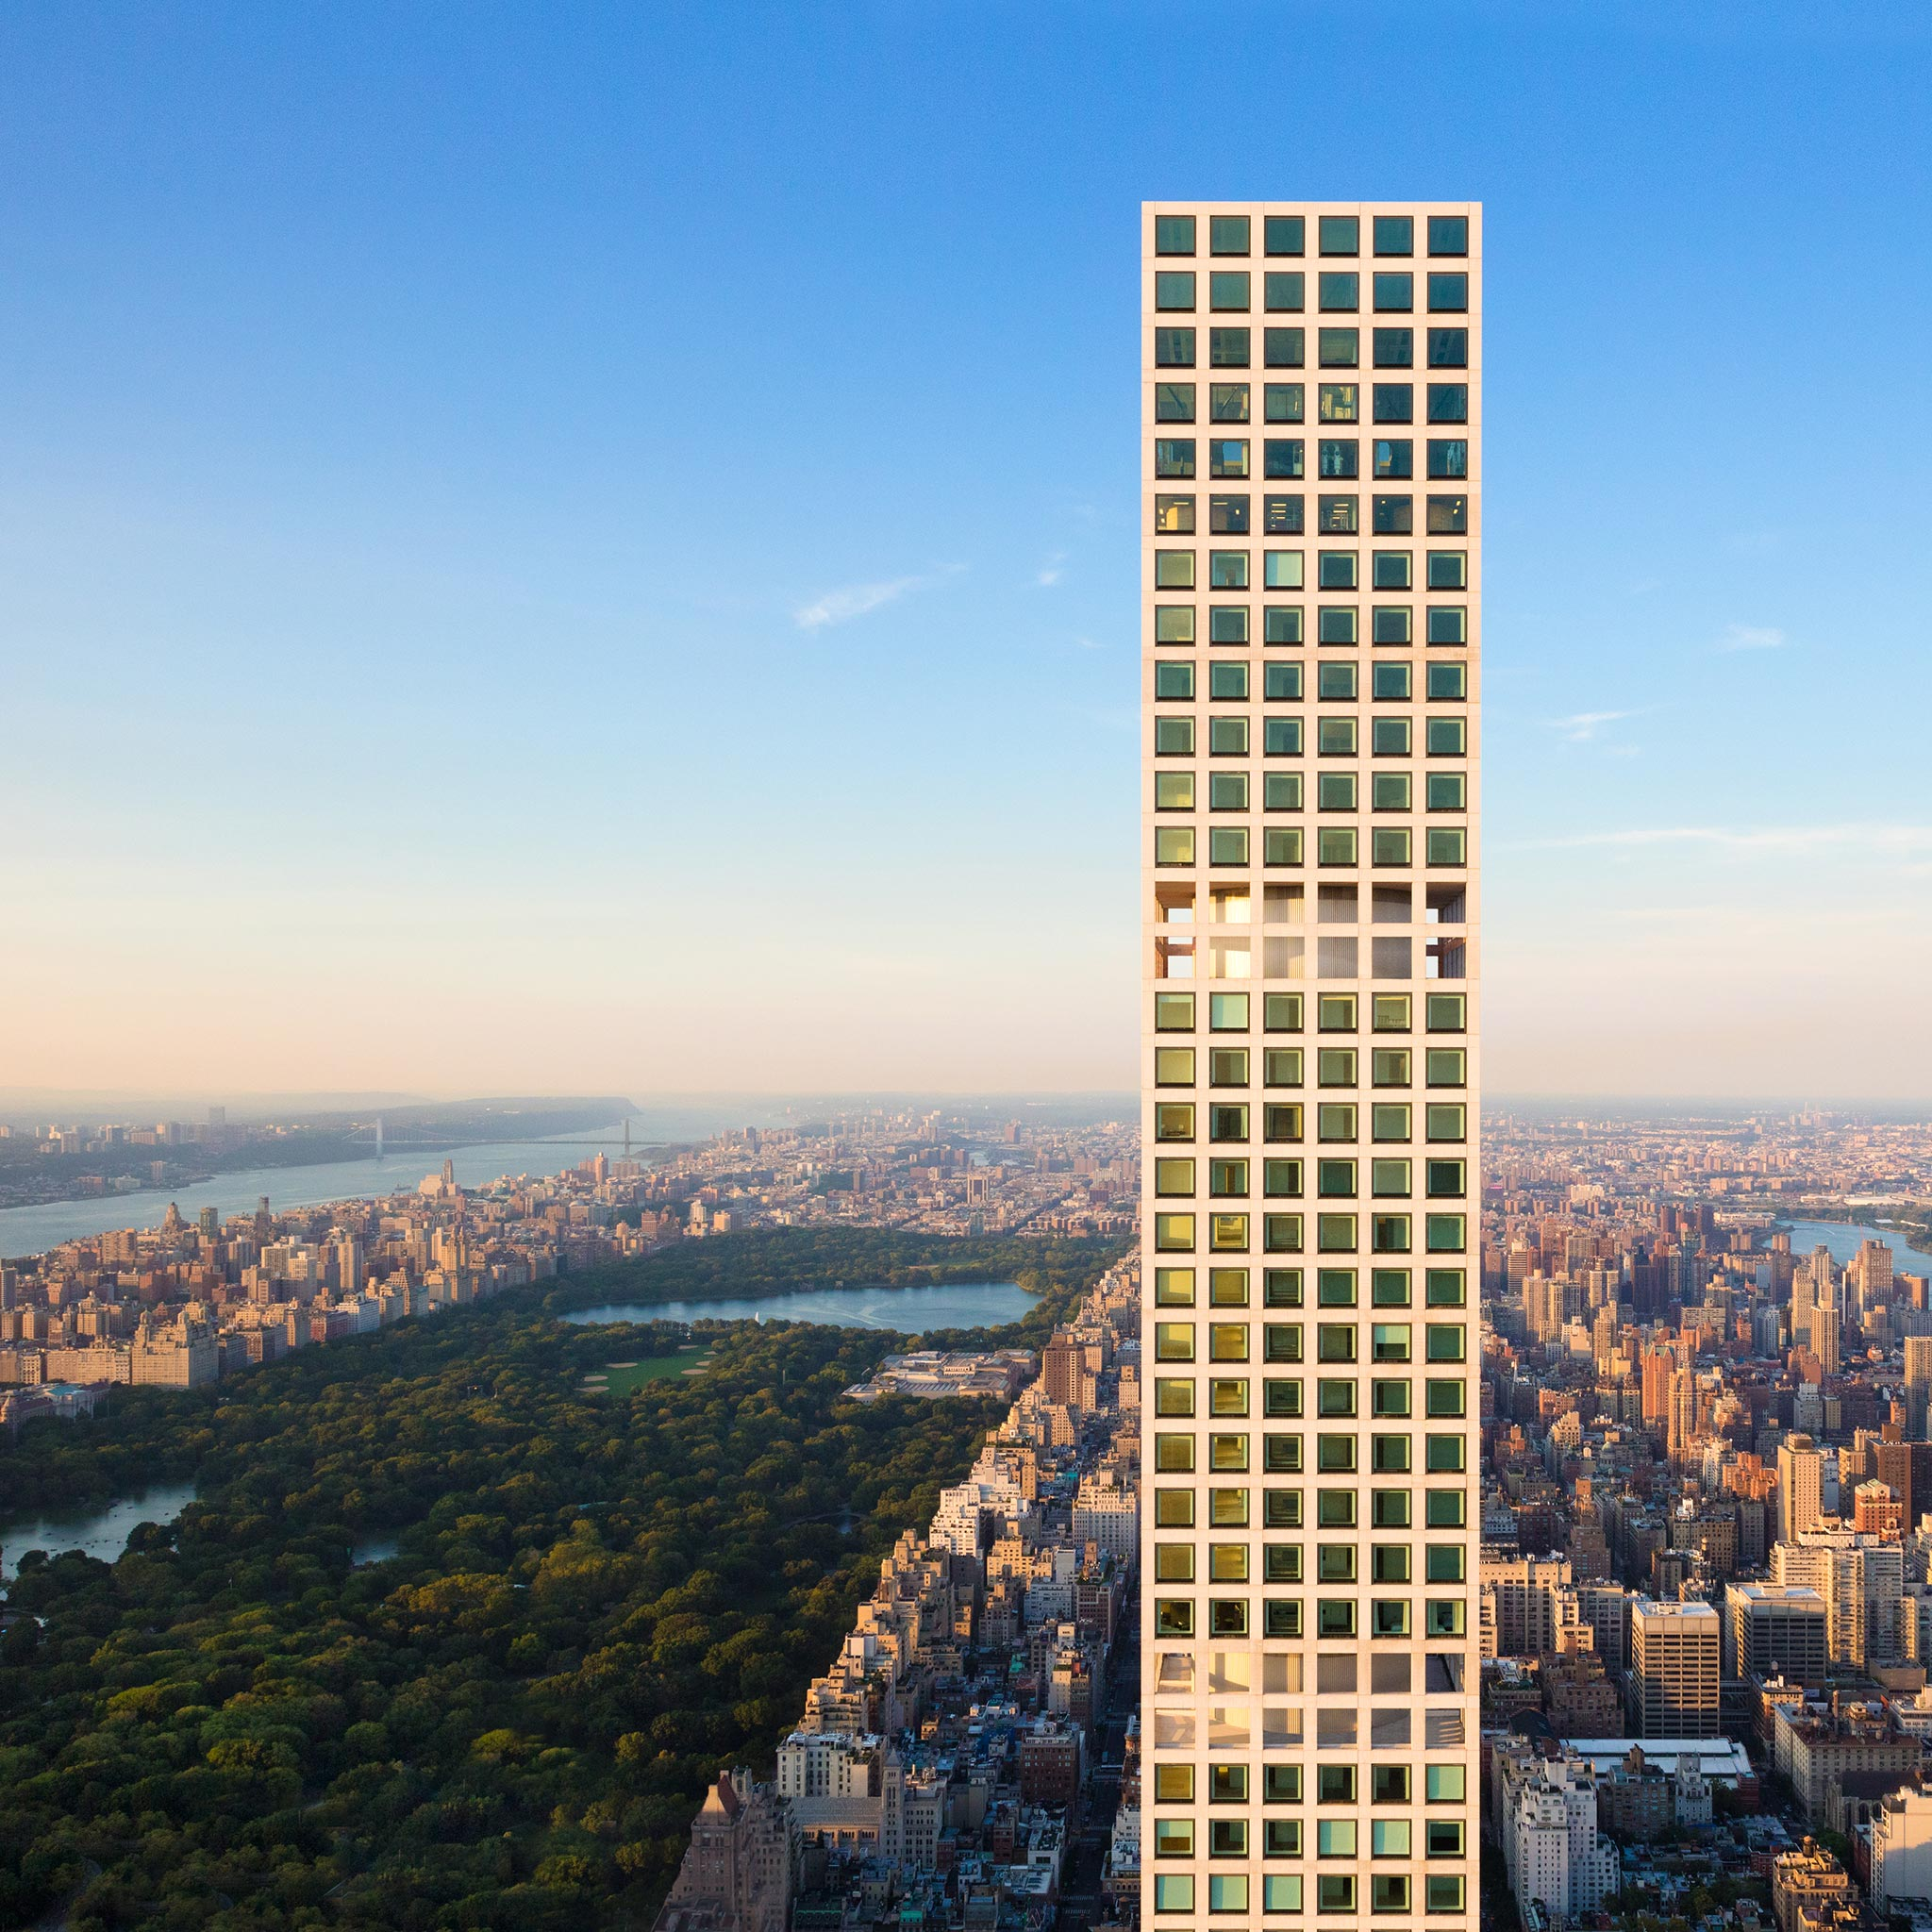
\includegraphics[width=11cm]{parkAvenue.jpg}
	\label{fig:Park_Avenue_432}
\end{figure}
\vfill

{
\renewcommand\arraystretch{2}
\begin{center}
\begin{tabular}{ >{\bf} l p{10cm} l }
Hochschule&Hochschule für Technik - FHNW\\
Studiengang&Elektro- und Informationstechnik\\
Autoren&Gruppe 4\\%Bachmann Lars \newline  Fischer Roni \newline Imhof Frank \newline Puschmann Pascal\\ 
Betreuer&Pascal Buchschacher \newline Anita Gertiser\\
Auftraggeber&Felix Jenni\\
Version&1.0 %Normally not used!
\end{tabular}
\end{center}
}

\clearpage
\documentclass[12pt]{article}
\title{Management Summary}

\begin{document}

\section*{Management Summary}
%------Problemstellung
%Worum ging es? Welches Problem sollte gelöst werden?
(FRANK) In Hochhäusern und Wolkenkratzern fliesst Abwasser von hoch oben nach unten. Die potentielle Energie, die das Wasser in den oberen Stockwerken hat, bleibt ungenutzt. Das Ziel der Gruppe 4 war, herauszufinden, ob und wie man diese potentielle Energie am besten nutzen könnte.\\
(MICHEL)


%------Vorgehen
%Wie sind Sie vorgegangen, um die Aufgabe zu lösen?
(FRANK) Von Beginn an hatte die Gruppe 4 den Lösungsansatz, mit einer Turbine im Abwasserrohr die Energie zu nutzen. Es entstanden aber insgesamt 4 verschiedene Lösungsansätze. Wie viel Energie die diese jeweils liefern könnten, berechnete die Gruppe 4 an einem Hochhausmodell. Durch eine Nutzwertanalyse wurden die Lösungen miteinander verglichen und so konnte ein Entscheid gefällt werden.\\
(MICHEL)


%------Hauptergebnisse
%Was sind die wesentlichen Ergebnisse – positive und negative Abweichungen?
(RONI)
(LARS)

%------Handlungsempfehlung
%In welcher Weise können die Ergebnisse verwendet werden? Welche Probleme bleiben ungelöst?
(PASCAL)
(LARS)
\end{document}

\documentclass[12pt]{article}
\title{Inhaltsverzeichnis}

\begin{document}
\renewcommand{\arraystretch}{2}
\section*{Inhaltsverzeichnis}
\begin{table}[H]
\huge
\begin{tabular}{p{14cm} p{1cm}}
1. Hauptteil&\\
\qquad 1.1 Auftrag des Arbeitgebers&\\
\qquad 1.2 Recherchedokument&\\
\qquad 1.3 Pflichtenheft - organisatorischer Teil&\\
\qquad 1.4 Pflichtenheft - technischer Teil&\\
\qquad 1.5 Aufbauorganisation&\\
2. Reflexion&\\
\end{tabular}
\end{table}
\end{document}

\begin{Huge}
1 Hauptteil: Dokumentation der Projektarbeit
\end{Huge}
\newpage
\begin{Huge}
1.1 Lastenheft/Aufgabenstellung
\end{Huge}
\newpage
\begin{Huge}
1.2 Recherchedokument
\end{Huge}
\newpage
\begin{Huge}
1.3 Pflichtenheft - organisatorischer Teil
\end{Huge}
\newpage
\begin{Huge}
1.4 Pflichtenheft - technischer Teil
\end{Huge}
\newpage
\begin{Huge}
1.5 Aufbauorganisation
\end{Huge}
\newpage
\begin{Huge}
2 Reflexion
\end{Huge}

\documentclass[12pt]{article}
\title{Reflexion}

\begin{document}

\section{Reflexion}



\end{document}

\end{document}
